\section{The Theory}

\subsection{Life ray}\index{Core Concepts@Core Concepts!life ray}

Every human being can be imagined as moving along a line -- a \textbf{life ray} -- which begins at birth and ends at death.
This ray represents the personal development, experience, and temporal unfolding of an individual within their \textit{own space}.

The life ray is not simply a timeline in the chronological sense.
It is the lived continuity of a person: their position in the world, their becoming, their self-story as it extends through time.

\subsection{Own Space and Shared Space}

The concept of the \textbf{own space}\index{Core Concepts@Core Concepts!own space}
own space (\textit{Eigenraum})\index{Core Concepts@Core Concepts!Eigenraum|see{own space}} is central to the model.
It denotes the interior dimension of existence — the personal, biographical, and perceptual world within which each life ray unfolds.
In the own space, experiences are not merely recorded but lived; they accumulate as fragments of meaning, memory, and identity.
The own space is invisible to others, yet it forms the hidden topology of the self.
Each person’s life ray moves within this internal continuum, unique and inaccessible from the outside.

The \textbf{shared space}\index{Core Concepts@Core Concepts!shared space} (\textit{gemeinsamer Raum})\index{Core Concepts@Core Concepts!gemeinsamer Raum|see{shared space}},
by contrast, emerges only when two or more own spaces come into relation.
It is not a neutral arena but a temporary projection — an \textit{image} of the individual life rays, translated into a common field of visibility.
Within this field, interactions become perceivable: gestures, words, movements, eye contact.
What meets in the shared space are not the totalities of two beings, but the projected outlines of their inner trajectories.
In this sense, the shared space is an externalized intersection of otherwise private worlds.

Crucially, the shared space functions as a bidirectional translator between interior and exterior.
From the own space outward, an individual projects expressions, intentions, and actions;
from the shared space inward, each participant receives impressions, emotions, and reflections.
What occurs outside is internalized as a fragment, transformed by interpretation and stored along the \textbf{life ray}.
Meaning thus arises not within either world alone, but through the oscillation between them.

The two spaces never perfectly coincide.
Every projection loses something of the original, every perception misaligns what was intended.
Yet it is precisely within this misalignment — this space of incompleteness — that human meaning, emotion, and memory are born.
The \textbf{shared space} is therefore both connection and difference:
a transient image of mutual presence that echoes back into the solitude of the \textbf{own space}.


\subsection{Shared space \& points of intersection}\index{Structural Relations@Structural Relations!intersection}

When two people meet, their \textbf{life rays} momentarily overlap in what I call a \textbf{shared space}.
Within that shared space, \textbf{points of intersection} are created:
concrete moments of encounter in which perception, attention, and presence mutually lock.

These intersection points are not just situations in the ordinary sense (``we talked in a hallway'').
They are structural events. They alter how each person is encoded in the other.

\subsection{Fragment formation}\index{Core Concepts@Core Concepts!fragment}

An intersection in the \textbf{shared space} is then carried back into the individual's
\textbf{own space} as a \textbf{fragment}: a unit of memory, impression, or imprint.
A \textbf{fragment} is a condensed biographical marker.
It may be faint, or it may be deeply formative.

In other words: encounters become \textbf{fragments}, and fragments become part of the chain of self.

Over time, a person accumulates many such \textbf{fragments}.
Arranged along the \textbf{life ray}, they form what can be called a
\textbf{fragment chain}\index{Core Concepts@Core Concepts!fragment chain} -- a chain of remembered contacts,
shaping identity not only by what happened, but by \textit{who} touched the ray and left something behind.

\subsection{Double helix \& emotional proximity}\index{Core Concepts@Core Concepts!emotional proximity}

When two people meet not just once, but repeatedly, or with unusual intensity, multiple
\textbf{intersection points}\index{Core Concepts@Core Concepts!intersection points} are formed.
In such cases, the two \textbf{life rays} begin to \textit{twist} around each other. Symbolically,
they approach the form of a \textbf{double helix}\index{Core Concepts@Core Concepts!double helix}:
two trajectories, entwined, mutually shaping.

In rare cases, this twisting can become so tight that what emerges is not merely two rays in proximity,
but a \textbf{temporary shared strand}\index{Core Concepts@Core Concepts!we-structure@we-structure (shared strand)} -- a lived ``we''-structure.
This is often how we experience deep friendship, romantic closeness, family bonds, or formative companionship.

The metaphor of ``\textbf{life rays}'' and their twisting into a double helix is not arbitrary. It echoes classical depictions of social systems,
in which intertwined structures represent the interdependence of individual and relational dynamics (see Figure~\ref{fig:doppelhelix}).

\begin{figure}[h]
    \centering
    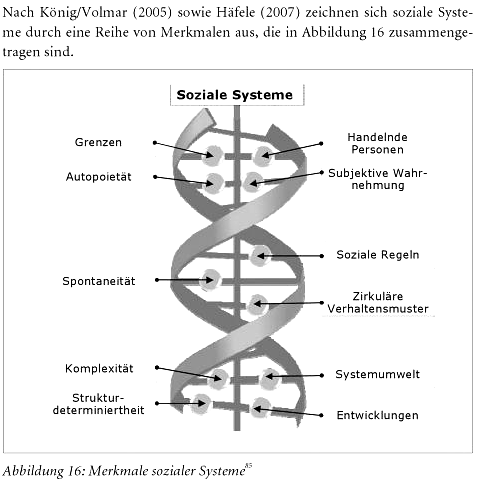
\includegraphics[width=0.7\textwidth]{figures/Doppelhelix.png}
    \caption{Characteristics of social systems represented as a double helix, adapted from \protect\cite{bartscher2011}, following König, Volmer, Häfele.}
    \label{fig:doppelhelix}
\end{figure}

\subsection{Relation to Existing Theoretical Frameworks}

While the Life Ray Theory resonates with several established traditions, it is not intended as a reformulation of any single existing framework.

Phenomenological approaches, such as those of Merleau-Ponty, inform the emphasis on \textit{lived appearance} and \textit{perceptual presence}, but the present model
does not remain at the level of description. Instead, it introduces explicit structural elements -- \textbf{life rays}, \textbf{fragments},
and \textbf{fragment chains} -- that allow phenomenological insights to be translated into relational configurations.

Narrative theories of identity, notably Ricoeur’s work, parallel the idea that identity emerges through \textit{temporally ordered meaning}. However,
the \textbf{fragment chain} model replaces narrative continuity with a discrete, \textit{event-based} structure, emphasizing accumulation and resonance rather than
coherent storytelling.

Systems-theoretical perspectives, including Luhmann’s, inspire the treatment of encounters as \textit{coupling events}. Yet the \textbf{life ray} Theory
retains subjectivity as the \textit{primary locus of meaning formation}, rather than dissolving it into purely systemic operations.

Accordingly, the present framework should be understood as a structural–phenomenological \textit{synthesis}: it offers a new topological
language for encounter and memory formation that is compatible with, but not reducible to, existing theories.
